\documentclass[12pt]{article}
\usepackage[a4paper, margin=2cm]{geometry}
\usepackage[english]{babel} % To obtain English text with the blindtext package
\usepackage{blindtext}
\usepackage{graphicx} % Required for inserting images
\usepackage{array, multirow} % For extra column formatting
\usepackage{amsmath, amssymb} %for equation environment
\usepackage{float}
\usepackage{parskip} % For gaps between para
\usepackage{setspace}
\usepackage{pdfpages}
\usepackage{abstract}
\usepackage[export]{adjustbox}
\usepackage{emptypage}
\usepackage{tocloft}
\usepackage[nottoc]{tocbibind}
\usepackage{hyperref, url}
\usepackage[table]{xcolor}
\usepackage{minted}
    \usemintedstyle{monokai}
\usepackage{caption}
    \captionsetup{font=footnotesize,labelfont=bf}
\usepackage{tcolorbox}
    \newtcolorbox{mintedbox}{
        colback=backcolour,
        boxrule=0pt,
        sharp corners,
        width=\linewidth,
        left=0pt, right=0pt,
        top=3pt, bottom=3pt
    }

\cftsetindents{section}{0em}{2em}
\cftsetindents{subsection}{0em}{2em}

\renewcommand\cfttoctitlefont{\hfill\Large\bfseries}
\renewcommand\cftaftertoctitle{\hfill\mbox{}}

\graphicspath{ {./images/} }

\pagenumbering{arabic}

\definecolor{blurple}{HTML}{5865F2}
\definecolor{backcolour}{HTML}{272823}

\hypersetup{
    colorlinks=true,
    linkcolor=black,
    urlcolor=blurple,
    citecolor=blurple,
}

\urlstyle{same}

\renewcommand{\arraystretch}{1.3}

\setcounter{secnumdepth}{5}
\setcounter{tocdepth}{5}
\newcommand\simpleparagraph[1]{%
  \stepcounter{paragraph}\paragraph*{\theparagraph\quad{}#1}}

%%%%%%%%%%%%%%%%%%%%%%%%%%%%%%%%%%%


\title{PHYC20040 Exp.2 Pleiades SM}
\author{Joana Adao}
\date{\today}

\begin{document}

\begin{titlepage}
    \begin{center}

        \begin{figure}[ht]
            
\includegraphics[width=\textwidth]{UCDLogo.png}
        \end{figure}
        
        \begin{figure}
            \centerline{
\includegraphics[width=\paperwidth]{UCDBanner.png}}
        \end{figure}

        \vspace{4cm}

        {\LARGE \bfseries PHYC20040 Exploring the Solar System}\\
        \vspace{0.75cm}
        {\Large Experiment No.2 Photoelectric Photometry of the Pleiades}
        
        \vspace{1cm}
    
    {\Large \textbf{12 February 2025}}

    \vspace{2cm}
    
    {\large \textbf{by Joana C.C. Adao (Student No. 23311051)}}\\

    \end{center}
    
   \clearpage

\end{titlepage}

\setcounter{page}{1}
\tableofcontents

\newpage

\begin{abstract}
\addcontentsline{toc}{section}{Abstract}

The aim of this experiment was 

\end{abstract}

%%%%%%%%%%%%%%%%%%%%%%%%%%%%%%%%%%%

\section{Theory} \label{sec:1}

Photometry plays an important role when it comes to astronomy and measuring different properties of stars, such as brightness and temperature.
UBV Photometry and its consequent B-V colour index have greatly defined what it means to determine stellar classifications, leading to the development
of the H-R Diagram with a focus on main-sequence stars. This experiment focuses on the study of the Pleiades cluster by comparing the calculated
apparent magnitudes to the known absolute magnitudes and luminosity of the main sequence stars.

\subsection{Photometry} \label{sec:1.1}

\textbf{Photometry} is a measurement of the brightness of celestial objects, such as stars and planets, that give astronomers access to that celestial object's composition,
temperature, distance, age, and more
\cite{britphoto}.
It is a special subset of radiometry which measures light waves by the typical response of the average human eye
\cite{mictechphoto, photophoto}.

Photometry has some fundamental quantities that aid in understanding what is being measured \cite{WYATT197815,photophoto}:

\begin{itemize}
    \item \textbf{Luminous flux} is the visible light per second that the source radiates. It is measured with \textit{lumens} given by \textit{Watts}.
    \item \textbf{Luminous intensity}, directly related to the luminous flux, is the lumens per unit solid angle emitted. Originally known as 'candlepower', the unit of measurement
    is \textit{candela} given by \textit{Watts per steradian}.
    \item \textbf{Illuminance} is the measurement of the level of light at a particular surface. The unit of measurement is \textit{footcandle (English)} or \textit{lux (Metric)} which is
    given by \textit{Watts per square metre}.
    \item \textbf{Luminance} is what measures the apparent magnitude (brigthness) (see §\ref{sec:1.1.3}), it is the luminous flux that is emitted from a surface.
    It is therefore measured with the unit \textit{footlambert (English)} or \textit{candela per square metre (Metric)}, given be \textit{Watt/steradian/}$m^2$.
    The human eye is the most commonly-known luminance detector, of which the sensitivity to light, and therefore colour, can be seen in figure {\ref{fig:1}}.
    \item \textbf{Luminosity} is a measure of the intrinsic brightness (absolute magnitude) of a star, measured in \textit{Watts}, mostly compared to the Sun's luminosity \cite{cosmoslumi}.
\end{itemize}

\begin{figure}[H]
    \centering
    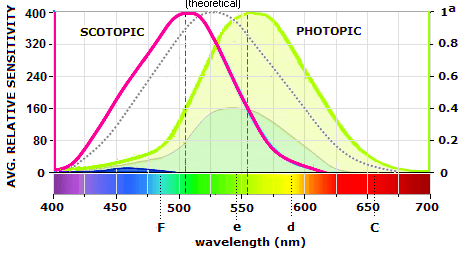
\includegraphics[width=12.5cm]{eye spectra curve.png}
    \caption{\centering Curve of the spectral sensitivity of the human eye \protect\cite{eyecurve}. \textit{Scotopic: very low light levels; Photopic: bright light levels \protect\cite{scophoto}.}}
    \label{fig:1}
\end{figure}

\subsubsection{UBV Photometry} \label{sec:1.1.1}

The UBV (Ultraviolet, Blue, Visual) classification system was originally called the Johnson-Morgan after H.L. Johnson and W.W. Morgan proposed this system for classifying stars in 1952 in accordance to their colour 
(and therefore temperature)
\cite{ubv1953}.
The apparent magnitudes of stars are measured in the three aforementiones wavelength bands and their spectral types are through the associated B-V (blue filter) and U-B (Ultraviolet filter)
(\textit{the difference between the magnitudes through the different filters}) colour indices
\cite{ubv1953}.

\begin{figure}[H]
    \centering
    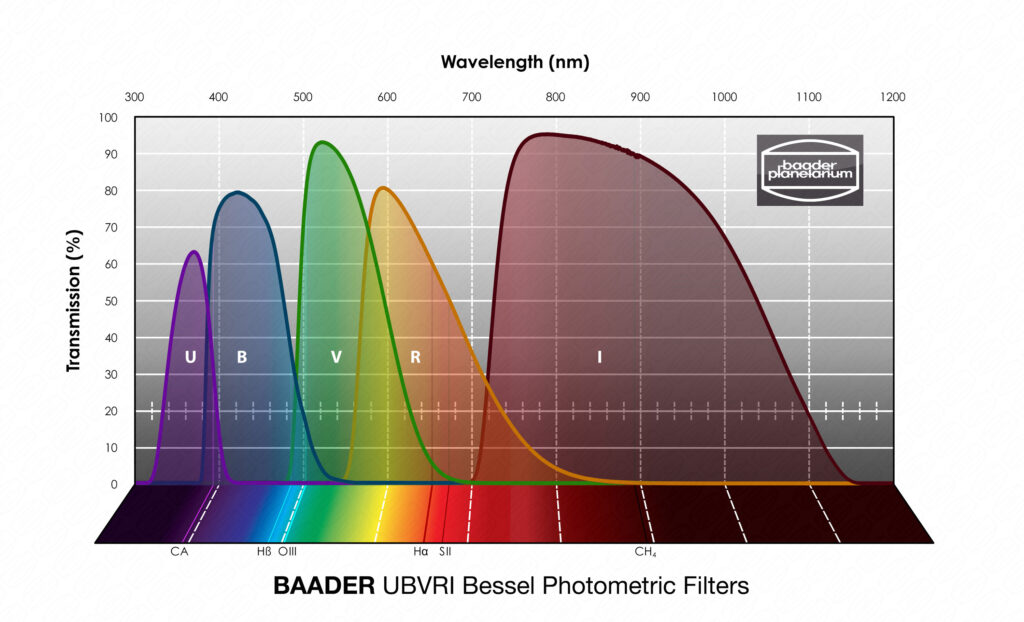
\includegraphics[width=12.5cm]{ubv.jpeg}
    \caption{\centering Transmission curves of photometric filters \protect\cite{ubvfilters}. \textit{U: Ultraviolet; B: Blue; V: Visible; R: Red; I: Infrared.}}
    \label{fig:ubvfilters}
\end{figure}

The UBVRI system above is an extension of the original Johnson-Morgan system with the extra red and infrared filters, allowing for a greater wavelength band allowance.

\subsubsection{The B-V Colour Index} \label{sec:1.1.2}

Colour, in astronomy, is defined as the difference in magnitude between two filters/wavelength bands, which is related to intensity logarithmically, 
\cite{sdsscolour,rochcolour,librecolour} such as B-V and U-B discussed in the previous section, §\ref{sec:1.1.1}.

On the flat, spanning z-axis of figure \ref{fig:ubvfilters} the B-V colour index (\textit{left}) that encompasses the range of visible light can be seen.

\subsubsection{Apparent and Absolute Magnitude} \label{sec:1.1.3}

Magnitude is a measure of the brightness of a star or other celestial body. The brighter the object, the lower the magnitude (number)
\cite{britmag}.
The magnitude of the celestial objects are divided into two types of observation:

\begin{itemize}
    \item \textbf{Apparent magnitude, m,} is used to describe how bright a celestial object appears from the view on Earth. Some of the brightest objects we can see
    have \textit{negative} apparent magnitude values (Sun = -26.7, Pluto (at brightest) = +13.7, for reference), meaning that they are particularly bright.
    \cite{lcomag}.
    \item \textbf{Absolute magnitude, M,} is defined as the magnitude of the star if the distance between it and Earth were 10 parsecs (pc)
    \cite{lcoabsmag,cosmosabsmag}.
    When at a set distance, astronomers are then able to compare intrinsic brightness of stars. The absolute magnitude refers to the absolute 'visual' magnitude, which restricts
    the measurement of the brightness to wavelength (4000 - 7000 Å)
    \cite{cosmosabsmag}.
    These magnitudes can also be negative values for particularly bright stars.
\end{itemize}

Absolute (\textbf{M}) and apparent (\textbf{m}) magnitudes can be used using equation \ref{eq:1} to calculate \textbf{D}, the distance in parsecs (pc). The magnitudes do not have units.
The distance modulus is then $\mathbf{m - M}$
\cite{cosmosabsmag}.

\vspace{-1.5ex}
\begin{gather} \label{eq:1}
    M = m + 5 - 5 (\log_{10} D) \quad , \quad m - M = 5 \log_{10} \left( \frac{D}{10} \right)
\end{gather}

The above equation (\ref{eq:1}) can be manipulated to find the distance, \textbf{D}:

\vspace{-1.5ex}
\begin{gather} \label{eq:2}
    \log_{10}D = \frac{m - M + 5}{5} \quad \implies \quad D = 10^{\frac{m - M + 5}{5}}
\end{gather}

\paragraph{The Link Between Magnitude and Photometry} \label{sec:1.1.3.1} has already been mentioned is sections §\ref{sec:1.1.1} and §\ref{sec:1.1.2}.

The zero point, a starting place for reference, was picked to be the star Vega, of which the magnitude is now defined to be $0.0$.
The apparent magnitudes are related to the flux of the star in such a way that equation \ref{eq:1} can be written to account for the flux (F) \cite{ccds}:

\vspace{-1.5ex}
\begin{gather} \label{eq:3}
    m_1 - m_2 = -2.5 \log_{10}\left(\frac{F_1}{F_2}\right) \qquad ; \qquad m_1 = -2.5 \log_{10}\left(\frac{F_1}{F_{Vega}}\right)
\end{gather}

Thus, the magnitudes can be interpreted as the logarithm of the flux.
Absolute magnitude, in contrast, is related to the luminosity (true brightness) of an object
\cite{ccds}.
The H-R Diagram, covered in §\ref{sec:1.2}, makes use of this relation.

\paragraph{The Link Between Magnitude and Colour} \label{sec:1.1.3.2} is what is explored further in this report.

The B-V colour index (see §\ref{sec:1.1.2}) is actually calculated by the difference in the apparent magnitudes as measured by the Blue (B) and Visual (V) filters
for the UBV photometric system \cite{ccds}:

\vspace{-1.5ex}
\begin{gather} \label{eq:4}
    B-V = m_B - m_V = -2.5 \log_{10}\left( \frac{f_B}{f_V} \right) + \text{constant}
\end{gather}

In which the non-zero constant is added due to the way the 0.0 colour (Vega) is defined. Thus is can be understood that bluer (hotter) stars have a negative colour
in comparison to Vega, and redder (colder) stars have a poisitive colour
\cite{ccds}.

\subsection{Hertzsprung-Russel (H-R) Diagram} \label{sec:1.2}

The Hertzsprung-Russel (H-R) diagram plots the absolute magnitudes (see §\ref{sec:1.1.3}) against the temperatures (spectral types) of different stars \cite{brithr}.
Figure \ref{fig:hrdiagram} also includes the luminosity (see §\ref{sec:1.1}) and B-V colour (see §\ref{sec:1.1.2}) as axes on the graph.
The 0.0 base point of the star Vega as discussed in sections §\ref{sec:1.1.3.1} and §\ref{sec:1.1.3.2} is included to the far left of the bottom y-axis.

\begin{figure}[H]
    \centering
    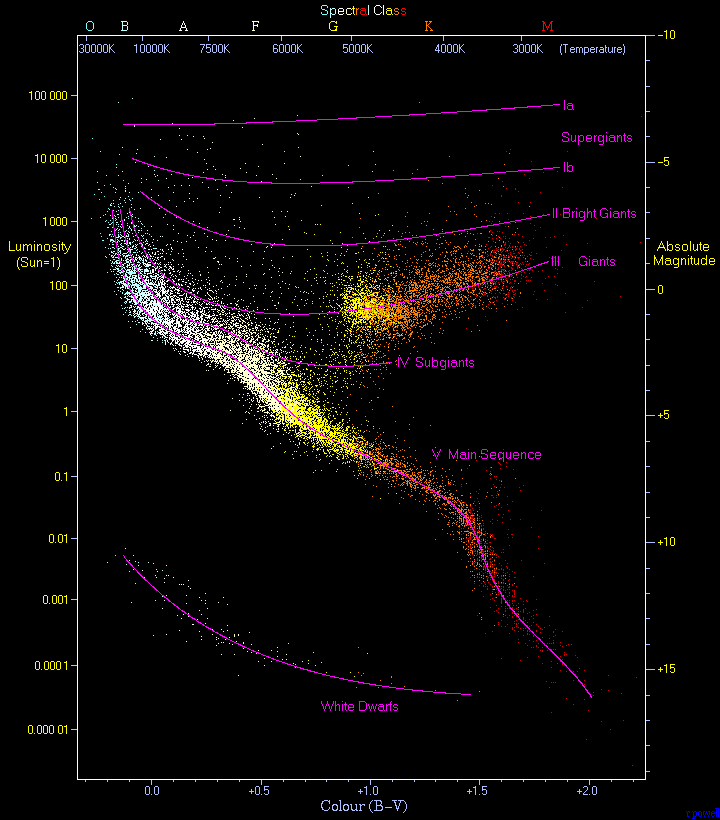
\includegraphics[width=10cm]{HRDiagram.png}
    \caption{\centering The Hertzsprung-Russell Diagram with 22 000 stars plotted in different regions highlighted accordingly \protect\cite{wikihr}.}
    \label{fig:hrdiagram}
\end{figure}

Astronomers can then use this diagram to be able to understand a star's internal structure and composition by determining its position on it \cite{cosmoshr,brithr}.
The way in which the stars scattered along the H-R diagram allowed astronomers to dictate the different regions, with the Main Sequence stars running diagonally across as
the most prominent and the gaints clustered above them in the diagram \cite{lcohr,cosmoshr}.

\subsubsection{Spectral Types} \label{sec:1.2.1}

The currently-used system of classification of stars was created by a team at Harvard in 1924 \cite{harvardstar}. The different classes are \textbf{OBAFGKM}, left to right: hottest to coldest.
The different classes and temperature thresholds are illustrated in figure \ref{fig:starclassy} with additional relevant information such as the (absorption) spectrum, the star colour, amount of hydrogen present, 
size in solar radii, and their prevalence (in percent) among the main sequence stars (see §\ref{sec:1.2.2})
\cite{lcostar,cosmosstar}.

\begin{figure}[H]
    \centering
    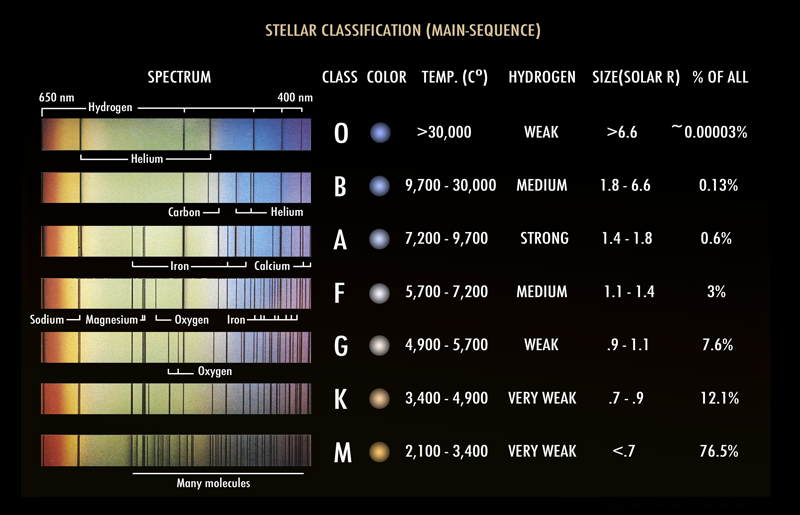
\includegraphics[width=12.5cm]{Stellar_Classification_Chart.png}
    \caption{\centering Chart for calssifying of the main star types as per the Harvard classification \protect\cite{wikistar}.}
    \label{fig:starclassy}
\end{figure}

The Sun is spectral type \textbf{G2} with temperature 5 700 K (Kelvin) \cite{cosmosstar}.

\subsubsection{Main Sequence Stars} \label{sec:1.2.2}

Main sequence stars are stars that undergo the fusion of hydrogen into helium at their core through nuclear reactions
\cite{schoolmsstar,studymsstar,nasamsstar}.
They are also defined by the way the radiation pressure from the nuclear reactions and the gravitational pressure work against each other in such a way that the star
remains stable \cite{studymsstar}; the process is known as \textbf{hydrostatic equilibrium} \cite{schoolmsstar}.

The relationship of a main sequence star with luminosity and temperature (spectral type) is seen in figure \ref{fig:hrdiagram}, the H-R diagram, and figure \ref{fig:starclassy},
the stellar type classification (for main sequence stars), which also shows the hydrogen available to undergo the nuclear reactions into helium.

\subsection{The Pleiades Star Cluster}

The Pleiades star cluster, also known as \textit{the Seven Sisters} and \textit{Messier (M) 45} and \textit{Cl Melotte 22}, can be found and seen by the naked eye near the shoulder of the Taurus (bull) constellation during Winter
\cite{nasapleiades,hubblepleiades}.
It is an open star cluster, in such that it contains thousands of stars that are loosely bound by gravity \cite{nasapleiades}.

Hubble telescope's Fine Guidance Sensors have estimated that the distance to the Pleiades from Earth is about \textbf{440 light-years} \cite{hubblepleiades} 
with an apparent magnitude of \textbf{1.6} \cite{sedspleiades,frenchpleiades}.

\begin{minipage}{.43\textwidth}
    \captionsetup{hypcap=false}
    \centering
    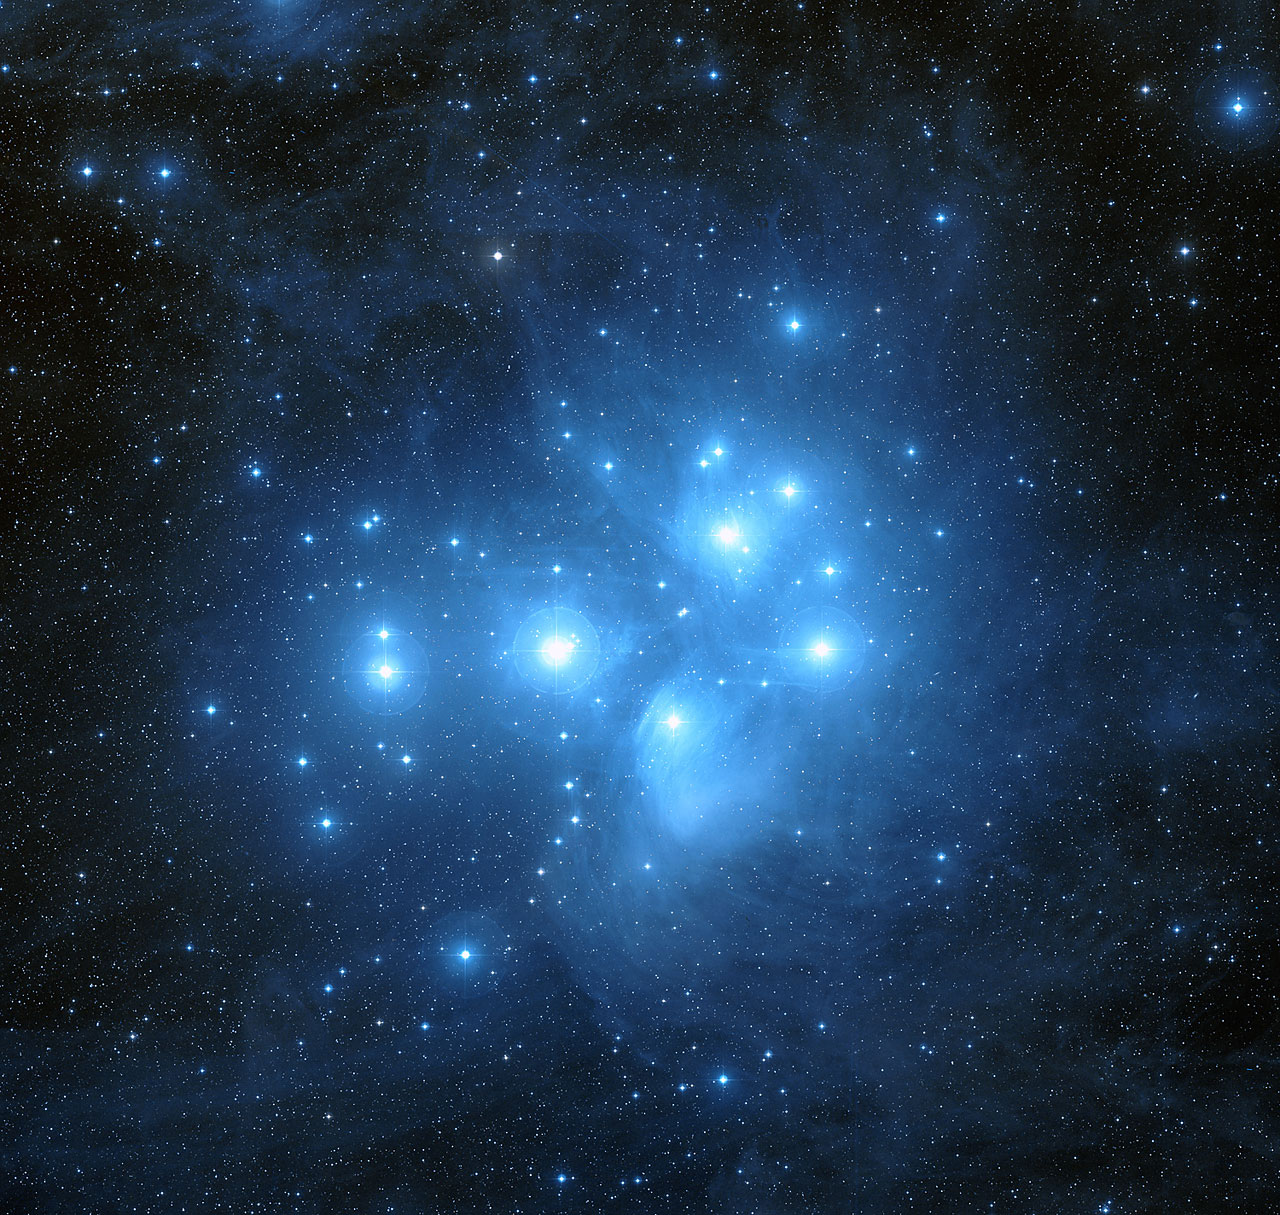
\includegraphics[width=\linewidth]{pleiades.jpg}
    \captionof{figure}{\centering Photo of the Pleiades/M45 \protect\cite{pleiades}.}
    \label{fig:plei}
\end{minipage}
\hfill
\begin{minipage}{.56\textwidth}
    \captionsetup{hypcap=false}
    \centering
    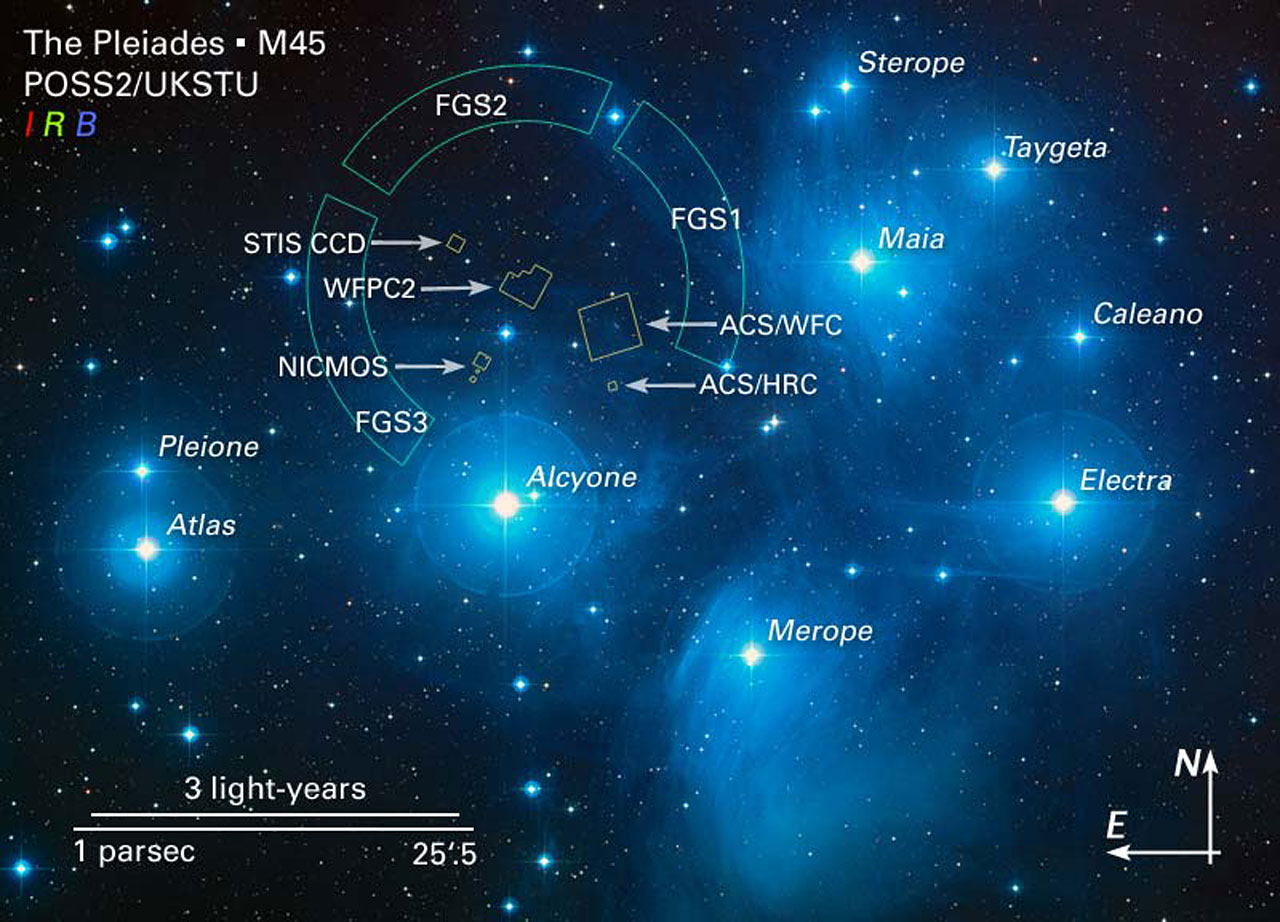
\includegraphics[width=\linewidth]{pleiades anotated.jpg}
    \captionof{figure}{\centering Annotated photo of the Pleiades/M45 \protect\cite{pleiadesann}.}
    \label{fig:pleiann}
\end{minipage}

Figure \ref{fig:plei} and figure \ref{fig:pleiann} are images sourced from the Hubble telescope of the Pleiades star cluster, with figure \ref{fig:pleiann} having the most visible stars named and labelled
and the Fine Guidance Sensors shown at the periphery of Hubble's field-of-view, tracing the circumference that is the approximate angular size of the Moon \cite{pleiadesann}.
A size/distance scale is also seen in the bottom left corner.

\section{Methodology} \label{sec:2}

This experiment made use of the \textit{Contemporary Laboratory Experience in Astronomy}, CLEA, software and the \textit{Photoelectric Photometry of the Pleiades} program included in the package.
CLEA is an online software developed to simulate and illustrate modern astronomical techniques in a 'real' night sky
\cite{cleasm}.

The program offered the simulated use of a UBV photometer attached to a 0.4m (16") research telescope. As the Earth rotates to the East in the program, the available "tracking" feature is used to essentially "stop"
the movement of the stars (West) in relation to the rotation of the Earth, allowing for the stable collection of data.

The apparent magnitude for two filters, Blue (B) and Visual (V), were found for 24 pre-determined stars as provided by the accompanying lab manual with the respective
right ascension (hours, minutes, seconds) and declination (degrees, minutes, seconds) coordinates attached \cite{UCDsm}.
These options and readings can be found on the left-hand side of the program, as shown in figure \ref{fig:program}.

\begin{figure}[H]
    \centering
    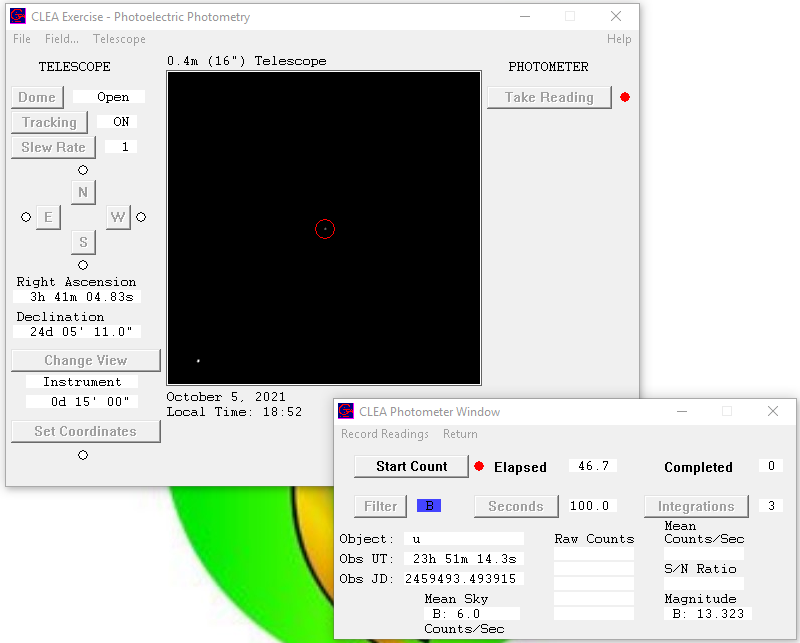
\includegraphics[width=.9\linewidth]{SMscreenshot_program.png}
    \caption{\centering Screenshot of the CLEA program in use.}
    \label{fig:program}
\end{figure}

Initial "sky" readings were taken for both filters (as seen in the separate, smaller window open in figure \ref{fig:program}) to account for the surrounding light not being emitted
from the studied star (true photon count is then \textit{star reading - sky reading}).

In addition to the \textbf{right ascension} and \textbf{declination} coordinates, which were provided, the following data was also noted and collected:

\begin{itemize}
    \item \textbf{Signal to Noise (S/N) Ratio} for both filter; fractional error.
    \item \textbf{Magnitude} (apparent) for both filters (B-V).
\end{itemize}

The uncertainties on the magnitude readings were minimised by ensuring the S/N ratio was greater than or at least 100 (70 for dimmer stars). This can be adjusted based on the amount of intergrations 
(number of times a measurement is repeated) doneand the seconds (how long light is collected for per integration) the photometer is allowed to collect data for. 

Dimmer stars generally needed more intergrations and longer seconds, with the maximum allowed to be done being: \textit{100 seconds, 5 intergrations}. This is approximately 8.5 minutes of photon collection.

With the collected data a H-R diagram can be plotted, with the apparent magnitude (V filter) and colour index (B-V), and compared against the accepted values of main sequence stars.

\section{Results and Calculations} \label{sec:3}

\begin{table}[H]

    \centering
    \caption{\centering Table of the values gathered for the Blue (B) and Visual (V) filter with respective S/N ratios, calculated B-V and corresponding S/N ratio included.}
    \resizebox{\textwidth}{!}{

        \begin{tabular}{|c|c|c|c|c|c|c|c|c|}
        \hline
        \textbf{Star} & \textbf{\begin{tabular}[c]{@{}c@{}}RA\\ hr min sec\end{tabular}} & \textbf{\begin{tabular}[c]{@{}c@{}}Dec\\ deg min sec\end{tabular}} & \textbf{B} & \textbf{\begin{tabular}[c]{@{}c@{}}S/N\\ (B)\end{tabular}} & \textbf{V} & \textbf{\begin{tabular}[c]{@{}c@{}}S/N\\ (V)\end{tabular}} & \textbf{B-V} & \textbf{\begin{tabular}[c]{@{}c@{}}S/N\\ (B-V) (\%)\end{tabular}} \\ \hline
        \textbf{1}    & 3  41  05                                                        & 24  05  11                                                         & 13.316     & 242                                                        & 12.513     & 352                                                        & 0.80         & 0.501                                                            \\ \hline
        \textbf{2}    & 3  42  15                                                        & 24  19  57                                                         & 4.200      & 6449                                                       & 4.310      & 6130                                                       & -0.11        & 0.023                                                            \\ \hline
        \textbf{3}    & 3  42  33                                                        & 24  18  55                                                         & 8.950      & 1774                                                       & 8.600      & 2085                                                       & 0.35         & 0.074                                                            \\ \hline
        \textbf{4}    & 3  42  41                                                        & 24  28  22                                                         & 10.250     & 975                                                        & 9.699      & 1258                                                       & 0.55         & 0.130                                                            \\ \hline
        \textbf{5}    & 3  43  08                                                        & 24  42  47                                                         & 13.058     & 271                                                        & 12.048     & 352                                                        & 1.01         & 0.466                                                            \\ \hline
        \textbf{6}    & 3  43  08                                                        & 25  00  46                                                         & 15.374     & 83                                                         & 14.365     & 133                                                        & 1.01         & 1.420                                                            \\ \hline
        \textbf{7}    & 3  43  39                                                        & 23  28  58                                                         & 8.468      & 404                                                        & 8.112      & 476                                                        & 0.36         & 0.325                                                            \\ \hline
        \textbf{8}    & 3  43  42                                                        & 23  20  34                                                         & 13.007     & 226                                                        & 12.023     & 356                                                        & 0.98         & 0.524                                                            \\ \hline
        \textbf{9}    & 3  43  56                                                        & 23  25  46                                                         & 11.162     & 524                                                        & 10.522     & 498                                                        & 0.64         & 0.277                                                            \\ \hline
        \textbf{10}   & 3  44  03                                                        & 24  25  54                                                         & 6.822      & 862                                                        & 6.800      & 871                                                        & 0.02         & 0.163                                                            \\ \hline
        \textbf{11}   & 3  44  11                                                        & 24  07  23                                                         & 9.931      & 357                                                        & 9.469      & 255                                                        & 0.46         & 0.482                                                            \\ \hline
        \textbf{12}   & 3  44  19                                                        & 24  14  16                                                         & 13.782     & 80                                                         & 12.630     & 136                                                        & 1.15         & 1.450                                                            \\ \hline
        \textbf{13}   & 3  44  27                                                        & 23  57  57                                                         & 2.780      & 5547                                                       & 2.870      & 5321                                                       & -0.09        & 0.026                                                            \\ \hline
        \textbf{14}   & 3  44  39                                                        & 23  27  17                                                         & 8.952      & 723                                                        & 7.720      & 988                                                        & 1.23         & 0.171                                                            \\ \hline
        \textbf{15}   & 3  44  39                                                        & 24  34  47                                                         & 17.032     & 79                                                         & 16.521     & 115                                                        & 0.51         & 1.536                                                            \\ \hline
        \textbf{16}   & 3  44  45                                                        & 23  24  52                                                         & 9.949      & 457                                                        & 8.802      & 775                                                        & 1.15         & 0.254                                                            \\ \hline
        \textbf{17}   & 3  45  09                                                        & 24  50  59                                                         & 8.162      & 465                                                        & 6.459      & 1018                                                       & 1.70         & 0.236                                                            \\ \hline
        \textbf{18}   & 3  45  27                                                        & 23  17  57                                                         & 5.380      & 1675                                                       & 5.450      & 1622                                                       & -0.07        & 0.086                                                            \\ \hline
        \textbf{19}   & 3  45  28                                                        & 23  53  41                                                         & 10.578     & 265                                                        & 10.018     & 343                                                        & 0.56         & 0.477                                                            \\ \hline
        \textbf{20}   & 3  45  33                                                        & 24  12  59                                                         & 7.070      & 544                                                        & 6.948      & 575                                                        & 0.12         & 0.253                                                            \\ \hline
        \textbf{21}   & 3  46  26                                                        & 23  41  11                                                         & 12.135     & 237                                                        & 11.351     & 241                                                        & 0.78         & 0.592                                                            \\ \hline
        \textbf{22}   & 3  46  26                                                        & 23  49  58                                                         & 16.807     & 82                                                         & 15.781     & 134                                                        & 1.03         & 1.430                                                            \\ \hline
        \textbf{23}   & 3  46  57                                                        & 24  04  51                                                         & 9.343      & 604                                                        & 9.168      & 507                                                        & 0.18         & 0.258                                                            \\ \hline
        \textbf{24}   & 3  47  29                                                        & 24  20  34                                                         & 7.550      & 1068                                                       & 7.421      & 655                                                        & 0.13         & 0.179                                                            \\ \hline
        \end{tabular}
    }
    \label{tab:1}
\end{table}

\section{Conclusion} \label{sec:4}


\newpage

%%%%%%%%%%%%%%%%%%%%%%%%%%%%%%%%%%%

\bibliographystyle{IEEEtran}
\bibliography{References} \label{sec:ref}

\vspace{1.5cm}

\listoffigures

\listoftables

\newpage

\section*{Appendix} \label{sec:A}
\addcontentsline{toc}{section}{Appendix}

\subsection*{Tables}
\addcontentsline{toc}{subsection}{Tables}

\begin{table}[H]
    \centering
    \caption{\centering Table of the provided data for the main sequence stars to be plotted \protect\cite{UCDsm, cleasm}.}

    \begin{tabular}{|c|c|c|}
    \hline
    \textbf{\begin{tabular}[c]{@{}c@{}}(V) Absolute\\ Magnitude\end{tabular}} & \textbf{B-V} & \textbf{Spectral Type} \\ \hline
    -5.8                                                                      & -0.35        & O5                     \\ \hline
    -4.1                                                                      & -0.31        & B0                     \\ \hline
    -1.1                                                                      & -0.16        & B5                     \\ \hline
    -0.7                                                                      & 00.0         & A0                     \\ \hline
    2.0                                                                       & 0.13         & A5                     \\ \hline
    2.6                                                                       & 0.27         & F0                     \\ \hline
    3.4                                                                       & 0.42         & F5                     \\ \hline
    4.4                                                                       & 0.58         & G0                     \\ \hline
    5.1                                                                       & 0.70         & G5                     \\ \hline
    5.9                                                                       & 0.89         & K0                     \\ \hline
    7.3                                                                       & 1.18         & K5                     \\ \hline
    9.0                                                                       & 1.45         & M0                     \\ \hline
    11.8                                                                      & 1.63         & M5                     \\ \hline
    16.0                                                                      & 1.80         & M8                     \\ \hline
    \end{tabular}
    \label{tab:2}
\end{table}

\subsection*{Code}
\addcontentsline{toc}{subsection}{Code}

\begin{center}

\begin{minipage}{\linewidth}
\captionsetup{hypcap=false}

\begin{mintedbox}
\begin{minted}[fontsize=\small, breaklines, baselinestretch=1.2, xleftmargin=0.5cm]{python}
import numpy as np

def errorprop(dx, dy): # error propagation defined formula
    error_x = 1 / dx
    error_y = 1 / dy

    return np.sqrt(error_x**2 + error_y**2)

B = np.array([13.316, 4.200, 8.950, 10.250, 13.058, 15.374, 8.468, 13.007, 11.162, 6.822, 9.931, 
            13.782, 2.780, 8.952, 17.032, 9.949, 8.162, 5.380, 10.578, 7.070, 12.135, 16.807, 9.343, 7.550])
sn_B = np.array([242, 6449, 1774, 975, 271, 83, 404, 226, 524, 862, 357, 80, 5547, 723, 79, 457, 
                465, 1675, 265, 544, 237, 82, 604, 1068])
V = np.array([12.513, 4.310, 8.600, 9.699, 12.048, 14.365, 8.112, 12.023, 10.522, 6.800, 9.469, 
            12.630, 2.870, 7.720, 16.521, 8.802, 6.459, 5.450, 10.018, 6.948, 11.351, 15.781, 9.168, 7.421])
sn_V = np.array([352, 6130, 2085, 1258, 352, 133, 476, 356, 498, 871, 255, 136, 5321, 988, 115, 
                775, 1018, 1622, 343, 575, 241, 134, 507, 655])

print(B-V)

print(errorprop(sn_B,sn_V)) # fractional error, since they're already put into fractions in the eqn
print(errorprop(sn_B,sn_V)*100) # percentage error

\end{minted}
\end{mintedbox}

\captionof{figure}{\centering Code used for table \ref{tab:1} in calculating the S/N ratio for B-V.}
\end{minipage}


\end{center}

\end{document}